\section{Background}
\label{sec:background}          

This section describes the building blocks we use to construct the
\datastruct.  We also describe related data structures, such as the
log-structured merge tree (LSM), in order to put our data-structural
innovations in context.  Finally, we summarize theoretical performance
analyses of the data structures.


%% \mfc{move to intro?}
%% \paragraph{Key-Value Operations.}

%% A \kv store implements the following operations:

%% \begin{relate}
%% \item[\textbf{Get(\emph{key})}:] Returns the \emph{value} associated with \emph{key}.
%% \item[\textbf{Insert(\emph{key},\emph{value})}:]  Inserts the pair \emph{key}/\emph{value},
%%   overwriting the old value if \emph{key} is already present.
%% \item[\textbf{Delete(\emph{key})}:] Removes \emph{key} and its associated
%%   \emph{value}. 
%% \item[\textbf{Range(\emph{key}$_1$,\emph{key}$_2$)}:] Return all
%%   key-value pairs \emph{k}-\emph{v} such that \emph{key}$_1 \leq $
%%   \emph{k} $\leq$ \emph{key}$_2$.

%% \end{relate}


\paragraph{The DAM model.}
We use the Disk Access Machine (DAM) model~\cite{DBLP:conf/icalp/AggarwalV87}
in our performance analyses.  In the DAM model, data is transferred between
disk and RAM of size $M$ in blocks of size $B$ words.  The I/O cost of a data
structure is the number of block transfers.
%When RAM becomes full, blocks may
%need to be written back to disk to make room for new blocks.
%Algorithms may manage the contents of RAM explicitly, or may use a
%paging algorithm, such as Least-Recently Used (LRU) to select blocks
%to be evicted.
%
%This model is used to analyze the IO efficiency of an algorithm or
%data structure, so t
%The DAM model is used to count the number of 
%primary performance metric is the number of
%block transfers performed by the algorithm or data structure and is
%predictive when an algorithm becomes IO bound.
In DAM model analyses, key-value pairs have size $O(1)$ words, so  the
write-amp 
of a key-value workload is
$\Theta(B\times W)$,
where $W$ is the amortized number of writes per insertion.

%Note
%that, when analyzing IO performance, we can completely ignore CPU
%costs.  Thus, for example, we often do not worry too much about the
%data layout within a block, since that only affects the CPU cost of
%searching or computing on the data in the block.


%\mfc{kill b-tree?}
\paragraph{B-trees.}
We analyze the write-amplification of B-trees to serve
as a baseline.
%We briefly review B-trees and their performance analysis in the DAM
%model~\footnote{Technically, we describe the B$^+$-tree.}.  A B-tree
%is an ordered search tree in which each node has size $B$, i.e. each
%node fits in exactly one block.  Internal nodes have fanout
%$\Theta(B)$ and depth $O(\log_B N)$.  Each leaf stores $\Theta(B)$
%key-value pairs.  Insertions and gets take $O(\log_B N)$ IOs in cold
%caches and $O(\log_B (N/M))$ if the cache is warm.  Range queries over
%$K$ items take $O(\log_B N + K/B)$ IOs in cold cache and $O(\log_B N/M
%+ K/B)$ IOs in warm cache.
Each insertion into a B-tree requires $\approx \log_B
N$\footnote{Throughout the paper, we use $\approx$ to indicate an
  analytical result accurate up to lower-order terms.  In other words,
  when we write $\approx X$, we mean $X+o(X)$.} writes in the worst
case, but almost all insertions modify only a leaf of the B-tree and
hence require only 1 write.
%, and modifications to the upper tree is a
%low-order term.
%.  To see why, observe that node
%splitting is a lower-order term of the I/O cost: each node split costs
%$O(1)$ I/Os and increases the number of nodes by 1, and the tree ends
%with $O(N/B)$ nodes, so splits contribute at most $O(N/B)$ I/Os,
%whereas writing a leaf for each insert costs $O(N)$ I/Os.  Thus the
%amortized writes per insertion is $O(1)$.
Although caching can help when the data set is small or the insertion
workload has locality, in the worst case of random inserts into a
large B-tree, each insertion will have to bring in a new leaf, causing
an old, dirty leaf to be written back to disk.  Thus the worst-case
write amplification of a B-tree is $\approx B$, much
greater than that of LSMs and \bets.

It is common to size the hardware so that all the indexing nodes of
the B-tree fit in RAM, i.e. RAM has size $M=N/B$.  In this case each
query and insert costs $O(1)$ I/O once the cache is warm.
%Caching does not significantly improve the worst-case write amplification of a B-tree.

%% To analyze the write amplification of a B-tree, notice that it is
%% sufficient analyze the write amplification of modifying leaves.
%% Although some copy-on-write implementations of B-trees modify all levels
%% of a tree when the leaf is modified, it is more efficient to use
%% an indirection table to only write modified nodes.  Furthermore, node
%% splits and merges incur a negligible cost, so we will neglect
%% it. Therefore, leaf modifications dominate.

%% If each insertion only changes one leaf, one might expect
%% the write amplification to be small.  However, changing one byte may
%% require writing an entire leaf, so the write amplification is $O(B)$,
%% which is prohibitive and explains why B-trees are implemented with
%% small nodes.

\paragraph{Log-structured Merge Trees.} 
%LSMs have inspired many variants, so 
%we first describe a generic LSM before discussing add-ons and
%optimizations.
A generic LSM consists of $k\approx \log_F \frac{N}{M}$ levels, $L_0,\ldots,
L_{k-1}$. Each level contains a sorted \defn{run} of key-value pairs.
The first run, $L_0$, has capacity $\Theta(M)$, and each subsequent
run has capacity $F$ times bigger than the previous. 
%Typical values
%of $F$ are in the range 2-10. 
The \defn{fanout} $F$ is a
parameter that trades off between insertion throughput and query
latency.  Each sorted run is called an \emph{SSTable}.

New items are inserted into $L_0$.  When an SSTable fills, it is
merged into the next table, which is called compaction. An SSTable can
receive $F$ such merges before it is full, so each element
participates in an average of $F/2$ compactions on a level before
being compacted into the next level.  Compaction is just a sequential
scan since both tables are sorted.  A compaction of total size $K$
takes $\approx K/B$ writes, or $\approx 1/B$ writes per key-value
pair, so the average write amplification is approximately
$\frac{F}{2}\log_F \frac{N}{M}$.  Assuming the cache has size $M=N/B$,
this simplifies to $\frac{F}{2}\log_F B$.

Most implementations also store indexing information about each
SSTable, so that queries in a table have similar performance to
queries in a B-tree.  Naively, a query in an LSM requires searching in
each level.  
%Searching in each level costs $O(\log_B N)$ I/Os, since each level is like a
%B-tree.
for a total cold-cache query cost of $O(\log_F \frac{N}{M} \log_B N)$
I/Os.  Given a warm cache of size $M=N/B$, we can cache the indexing
information of all the SSTables, so that each SSTable query requires
$O(1)$ I/Os.  Then, on a warm cache, the query cost becomes $O(\log_F
N/M)$, which is significantly higher than the $O(1)$ warm-cache query
in a B-tree given the same cache size.  This is for a generic LSM;
most LSM implementations use filters to reduce queries to $O(1)$ I/Os,
as described below.
%% Range queries take $O(\log_F N \log_2 N + K/B)$ IOs, since it is
%% basically a range query at each level, with an in-memory merge of the
%% resulting key-value pairs.  \mfc{warm cache}


%For typical values of $B$, $F$, and $N$,
%$\frac{F}{2}\log_F \frac{N}{M}$ is much smaller write
%amplification than the $\Theta(B)$ worst-case write amplification of B-trees.
%For example, if $F=2$, $N=2^{30}$, $M=2^{20}$ key-value pairs,
%and $B=1024$, the write amplification of an LSM is $\approx 10$,
%compared to $\approx 1024$ for a B-tree.
%% This analysis is surprisingly accurate.  For
%% example, the PebblesDB paper~\cite{!pebblesdb:raju} reported write amplifications in the
%% range from 27 to 42 for several LSMs on a dataset of size $2^{29}$
%% insertions.


%It is commonly stated that LSM trees have high write amplification.
%Although it's true that write amplification is a bottleneck to LSM
%insertion performance, they were actually a significant advance over
%B-trees in terms of worst-case write amplification.  However, if all insertions are to a
%small sub-tree, then a B-tree may be able to reduce its write
%amplification by caching the sub-tree.  A ``classic'' LSM tree, on the
%other hand, always does level-wide compactions, and so its write
%amplification, and hence its insertion throughput, are always the same
%as if the workload were purely random.  Thus, for some workloads, the
%write amplification of a B-tree may be less than that of an LSM tree.
%Some LSM trees include special cases for common workload patterns,
%such a sequential insertions or bulk loads.

An off-the-shelf LSM is typically
asymptotically much faster than a B-tree for insertions but, for some
insertion workloads that have high locality, can be asymptotically slower.  Queries can also be
asymptotically slower than in a B-tree, but this can largely be
mitigated with filters.

\paragraph{\Bets.} The generic \bet~\cite{DBLP:conf/soda/BrodalF03}
is
a B-tree that uses part of the space in each node to buffer items
recently inserted into the subtree rooted at that node.  Queries must
check for relevant mutations in each buffer along their search path.

Insertions place an item in the root node's buffer.  When the buffer
in a node becomes full, the \bet moves some of the
elements in the buffer to the buffer of one of its children.  The \bet
always moves items to the child that would be examined during a search
for those items, ensuring that a future query for one of those items
will find it. This process is called a \emph{flush} and is analogous
to an LSM compaction.  There are several options for how to select the
items to be flushed.  The most common policy is to select the child
for which the most items are buffered in the parent and then flush
all the items buffered for that child.  

To analyze the \bet in the DAM model, let $F\ll B$ be the fanout of
the \bet.\footnote{Historically $F = B^\epsilon$, where $0\leq
  \epsilon\leq 1$, which is where the name comes from.  We use $F$ to
  ease the comparison with LSMs.}  Thus pivots and child pointers
consume $O(F)$ space in each node.  The remaining $B-O(F)\approx B$
space in each node is used for buffering.  Thus the height of the tree
is $\approx\log_{F}N$ and the cold-cache query cost is
$\approx\log_F N$ I/Os.  

Each flush costs $O(1)$ I/Os and moves at least $B/F$ elements one
level down the tree.  Since each element moves at most $O(\log_F N)$
levels down the tree, insertions cost $O((F\log_F N)/B)$ amortized
IOs, which is the same as that of an LSM.  Likewise, the write
amplification of a \bet is $O(F\log_F N)$ without caching.

With a cache of size $M=N/B$, we can cache the top of the tree,
reducing query costs to $O(\log_F B)$ I/Os.  Insertions become
$O((F\log_F B)/B)$ I/Os, and write amplification reduces to
$O(F\log_F B)$, which are both the same as an LSM with the same size cache.

One advantage of \bets is that they can naturally exploit locality in the
insertion workload to improve insertion performance, much as a B-tree can.
This is because flushes are not done on a level-wide basis, but node by node.
Thus, for example, if a workload consists of insertions all destined for a
small sub-tree, a \bet can cache that sub-tree to reduce write amplification
and improve insertion throughput.

\paragraph{Filters.} Many LSM implementations mitigate the high
query cost of a generic LSM by using \defn{filters}; bloom filters~\cite{DBLP:journals/cacm/Bloom70} are the most well
known filters.
%A filter is a
%lossy, space-efficient set-membership data structure.  Filters have
%one-sided error: a query for an element in the set is guaranteed to
%return \texttt{present}, but a query for an element not in the set may
%erroneously return \texttt{present} with some \defn{false positive
%  probability} $\epsilon$.  
  The space requirement of a filter is $O(n
\log 1/\epsilon)$ for a set of a size $n$.  For typical values of
$\epsilon\approx 1\%$, this is about 1 or 2 bytes per element.
When filters are small enough to fit in RAM, they can reduce the I/O costs
of cold-cache point queries in LSMs to $O(\log_B N)$,
which is the same as in B-trees.  With a cache of size $M=N/B$,
queries cost $O(1)$ I/Os.  The same calculation holds for \bets. Note, however, that filters cannot
be used to speed up range queries, since filters do not support range
emptiness queries.

%Filters can also be used in \bets: each node is organized into a header,
%which contains pivots and a filter on the buffer contents, and a
%separately stored buffer.  The buffers are swapped in and out of
%memory as needed, but the headers are small and tend to stay in
%cache.  Then a \bet achieves the same bounds under the same
%assumptions as an LSM: $O(1)$ IOs for positive queries and
%no IOs for negative queries.

In our work we use a variant of quotient
filters~\cite{DBLP:journals/pvldb/BenderFJKKMMSSZ12}, because inserts and
lookups access only a constant number of distinct
locations~\cite{DBLP:journals/pvldb/BenderFJKKMMSSZ12}, making them generally
faster than Bloom filters.  Furthermore, quotient filters are, for the
false-positive rate used in \sysname, roughly the same size as Bloom filters.


% Besides size, the other main performance metric of a filter is cache
% misses.  In Bloom filters, the number of cache misses on a query is
% $O(\log 1/\epsilon)$ and in quotient filters, the number of cache
% misses is $O(1)$, with high probability.  In addition to being faster,
% quotient filters are 40\% smaller than Bloom filters and they support
% deletes and merging of filters.

% When the assumptions are violated, each data structure falls back to
% their its complexity.  RocksDB and PebblesDB use Bloom filters.
% Since the speed of NVMes force us to account for CPU and cache line
% miss costs, we will use quotient filters.

% \paragraph{Fractional Cascading.}
% In~\cite{!bender:streaming:oblivious}, Bender et 
% al.~introduced \emph{fractional cascading} as a way to reduce the
% query cost of LSMs, even for range queries.  In fractional cascading,
% pointers are added 
% between the sstables so that a search in one table can start in the
% next table without restarting the binary search from scratch.  They
% showed that fractional cascading can reduce the query cost in LSMs
% to match \bets.  
%\bets themselves naturally have pointers from level to level, so that
%on each level of the search tree only one node need be examined.

\paragraph{Size Tiering.} Cassandra introduced the notion of \emph{size
tiering} in an LSM.  In a size-tiered LSM (STLSM), each level has up
to $F$ SSTables of approximately the same size.  When a level
reaches its maximum number of SSTables, its SSTables are merged into
one SSTables, which is moved to the next level.
The advantage of size-tiering is that each item is involved in only
one compaction per level.  The downside is that queries now have
more places to search.

Kuszmaul~\cite{bradleywhitepaper} 
showed that with size tiering, write amplification decreases by a factor
of $F$ from that of a generic LSM to $O(\log_F
\frac{N}{M})$, while queries increase by a factor of $F$ to
$O(F \log_F \frac{N}{M} \log_B N)$ IOs.  Even if we assume
that the cache has size $M=N/B$, size tiering still trades off a
factor of $F$ reduction in write amplification for an
$F$-fold increase in query costs.  However, by maintaining a
filter for each SSTable on every level, the point query costs can be
kept at $O(1)$ IO per positive query and no IOs per negative query.
Size tiering also increases the costs of small range queries, and
filters don't mitigate that cost.

%% PebblesDB combined size tiering and skip-list-based fractional cascading.
%% They stress the importance of write amplification in key-value store
%% performance. Their results are consistent with Kuszmaul's theoretical
%% predictions.


% \mfc{looks like something to kill}

% \paragraph{The \wobtreeone.}
% The key innovation of the \wobtreeone is to use a B-tree to store the
% contents of each \bet node's buffer, as shown in \Cref{fig:wobtree}.
% The B-tree structure for the buffer makes searches within each node's
% buffer I/O-efficient.

% \begin{figure}[t]
%   \begin{center}
%     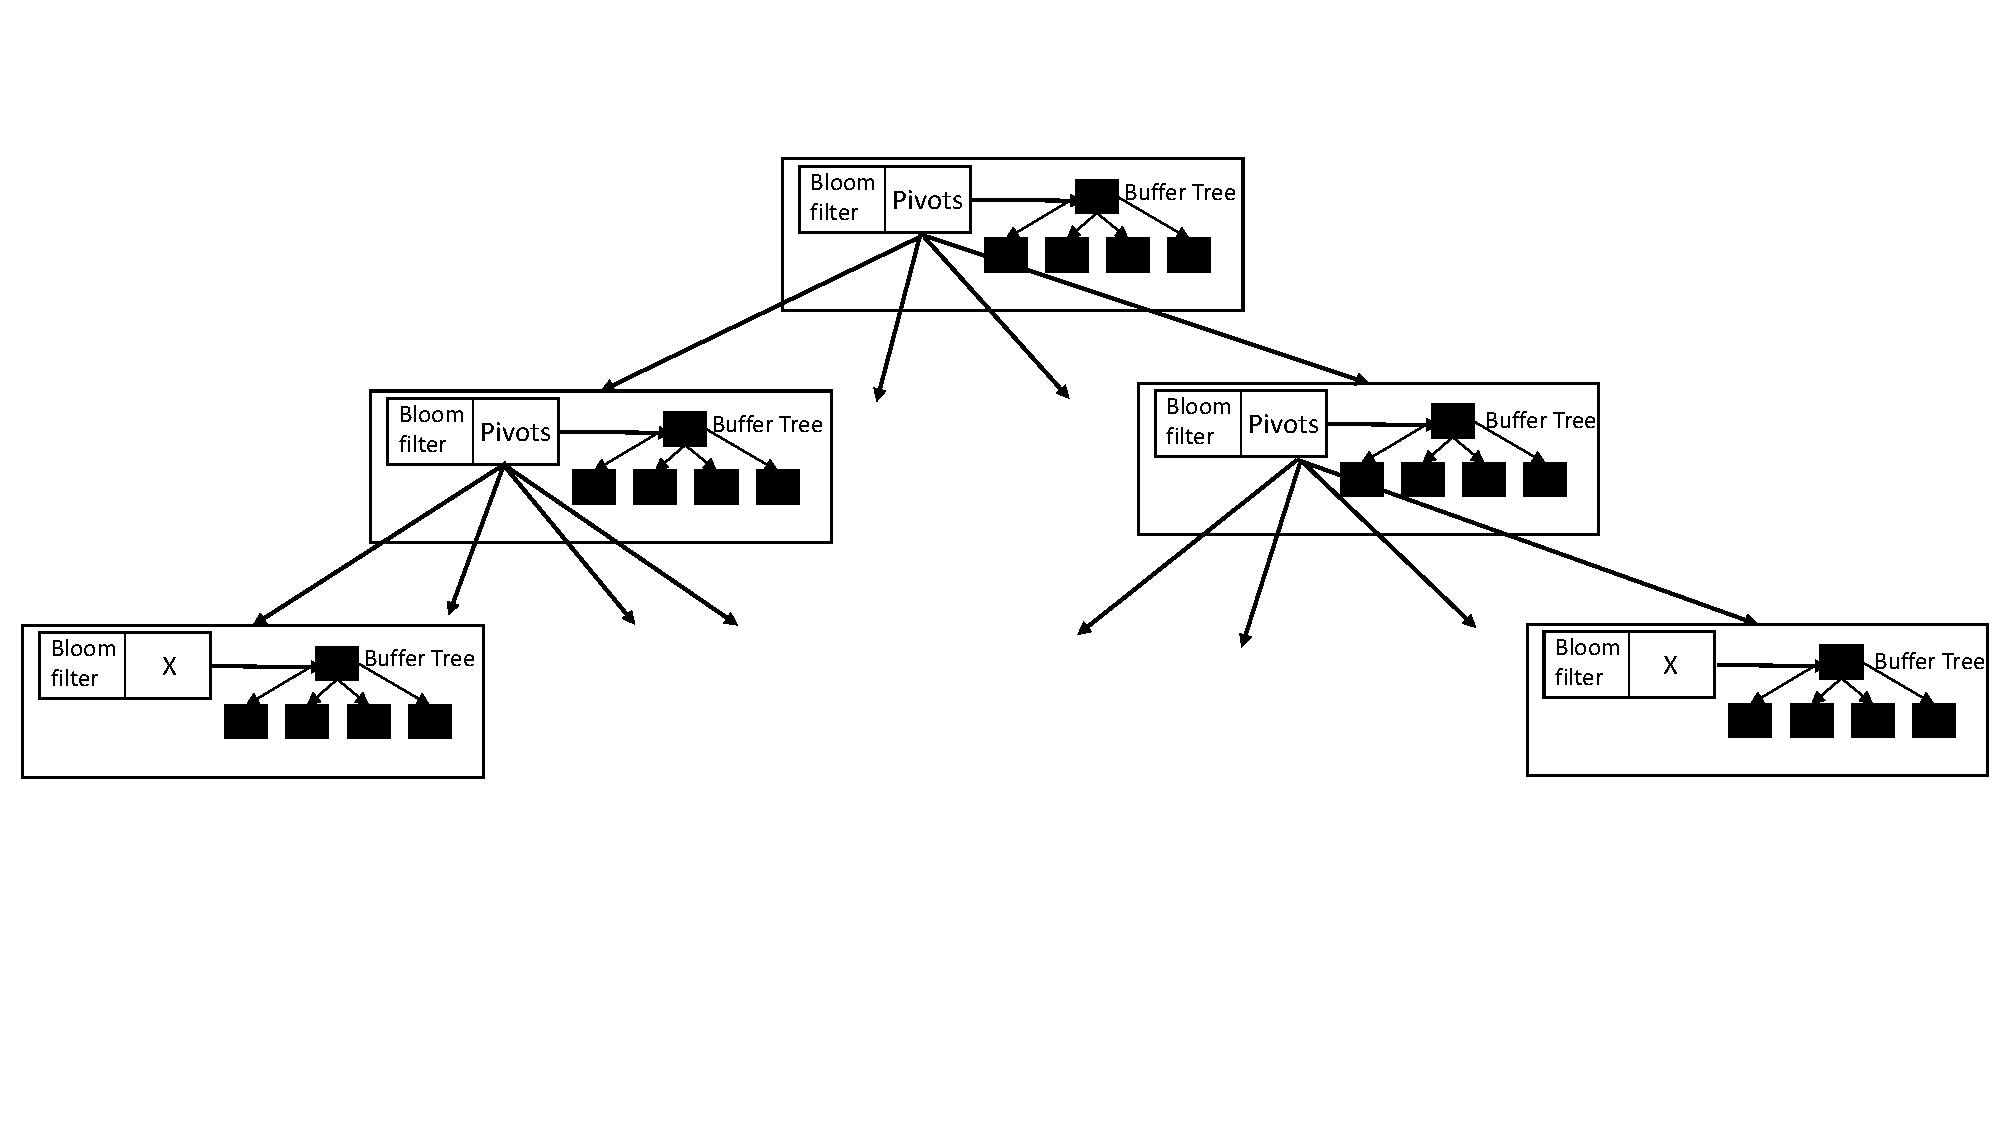
\includegraphics[scale=0.25]{wobtree.pdf}
%     \caption{The ``tree-of-trees'' \wobtreeone design.  Each \bet node
%       (indicated by white squares) stores its message buffer using a
%       B-tree (indicated by black squares).  The out square around each
%       \bet node and its buffer is purely illustrative---since this
%       data structure is designed for SSDs, there is no need to
%       maintain physical locality between a \bet node and the nodes of
%       its message buffer or between B-tree nodes belonging to the same
%       message buffer.}\label{fig:wobtree}
%   \end{center}
% \end{figure}

% The potential downside of using a B-tree is that, since the nodes of
% the B-tree might not be contiguous on disk, scanning the contents of a
% \bet node's buffer might require many disk I/Os.  However, the
% \wobtreeone is designed for SSDs, where locality is not so important
% as concurrency.  Thus, on SSDs, we can perform buffer scans at disk
% bandwidth, even if the B-tree nodes are not contiguous, by issueing
% multiple I/Os concurrently, so that the SSD always has a large number
% of I/O requests to serve concurrently (i.e. so that we maintain a high
% queue depth).
